\documentclass{article}

%w | ! clear; pdflatex %
%https://tex.stackexchange.com/questions/20784/which-package-can-be-used-to-draw-automata
%https://www3.nd.edu/~dchiang/teaching/theory/2018/www/tikz_tutorial.pdf
\usepackage[paperwidth=40 cm, paperheight=21cm, top=1cm,bottom=1cm,right=1cm,left=1cm]{geometry}
\usepackage{tikz, amsmath}
\usetikzlibrary{automata, positioning, arrows}

\begin{document}
\vspace*{0.5in}
{\bf\Large COMP 3602 Assignment 1}
\newline

Question 1a)

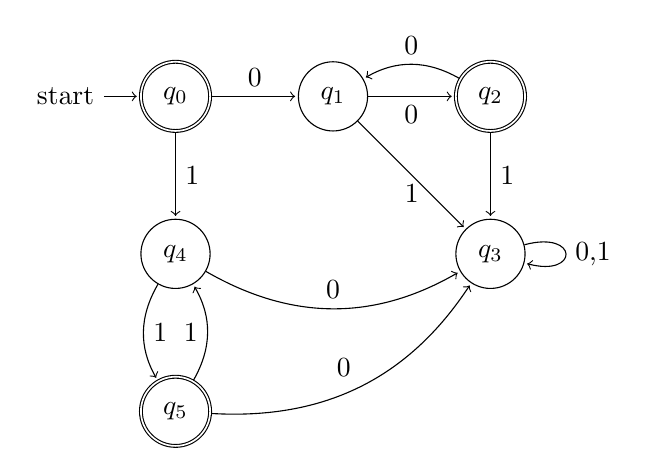
\begin{tikzpicture}[shorten >=1pt, node distance=2cm, on grid, auto]
    \node[state, initial, accepting] (q_0) {$q_0$};
    \node[state] (q_1) [right of = q_0] {$q_1$};
    \node[state, accepting] (q_2) [right of = q_1] {$q_2$};
    \node[state] (q_3) [below of = q_2] {$q_3$};
    \node[state] (q_4) [below of = q_0] {$q_4$};
    \node[state, accepting] (q_5) [below of = q_4] {$q_5$};
        \path[->]
        (q_0)   edge node {0} (q_1)
                edge node {1} (q_4)
        (q_1)   edge [below] node {0} (q_2)
                edge[below] node{1} (q_3)
        (q_2)   edge [bend right, above] node {0} (q_1)
                edge node {1} (q_3)
        (q_3)   edge [loop right] node {0,1} ()
        (q_4)   [bend right] edge node {1} (q_5)
                edge node {0} (q_3)
        (q_5)   [bend right] edge node {1} (q_4)
                edge node {0} (q_3);
\end{tikzpicture}

\vspace{2cm}

Question 1b)
\newline
\newline
\vspace{2cm}
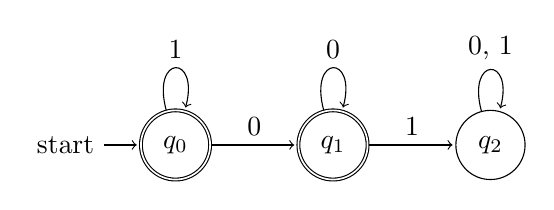
\begin{tikzpicture}[shorten >=1pt, node distance=2cm, on grid, auto]
    \node[state, initial, accepting] (q_0) {$q_0$};
    \node[state, accepting] (q_1) [right=of q_0] {$q_1$};
    \node[state] (q_2) [right=of q_1] {$q_2$};
        \path[->]
        (q_0)   edge node {0} (q_1)
                edge [loop above] node {1} ()
        (q_1)   edge node {1} (q_2)
                edge [loop above] node {0} ()
        (q_2)   edge [loop above] node {0, 1} ();

\end{tikzpicture}

\vspace{2cm}

\newpage
Question 2a)
\vspace{1cm}

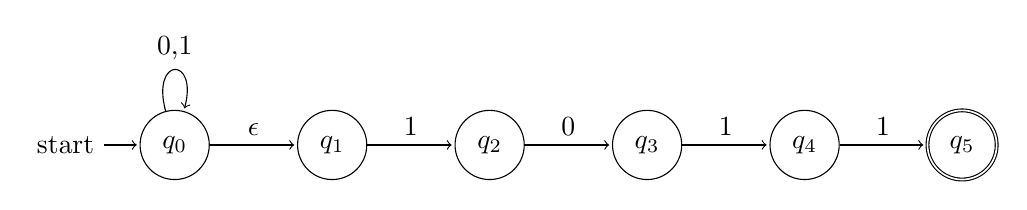
\begin{tikzpicture}[shorten >=1pt, node distance=2cm, on grid, auto]
    \node[state, initial] (q_0) {$q_0$};
    \node[state] (q_1) [right= of q_0] {$q_1$};
    \node[state] (q_2) [right= of q_1] {$q_2$};
    \node[state] (q_3) [right= of q_2] {$q_3$};
    \node[state] (q_4) [right= of q_3] {$q_4$};
    \node[state, accepting] (q_5) [right= of q_4] {$q_5$};
        \path[->]
        (q_0)   edge [loop above] node {0,1} ()
                edge node {$\epsilon$} (q_1)
        (q_1)   edge node {1} (q_2)
        (q_2)   edge node {0} (q_3)
        (q_3)   edge node {1} (q_4)
        (q_4)   edge node {1} (q_5);

\end{tikzpicture}

\vspace{2cm}
Question 2b)
\vspace{1cm}

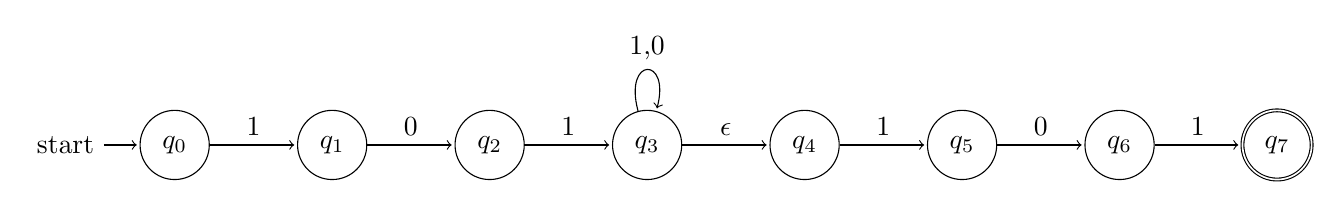
\begin{tikzpicture}[shorten >=1pt, node distance=2cm, on grid, auto]
    \node[state, initial] (q_0) {$q_0$};
    \node[state] (q_1) [right= of q_0] {$q_1$};
    \node[state] (q_2) [right= of q_1] {$q_2$};
    \node[state] (q_3) [right= of q_2] {$q_3$};
    \node[state] (q_4) [right= of q_3] {$q_4$};
    \node[state] (q_5) [right= of q_4] {$q_5$};
    \node[state] (q_6) [right= of q_5] {$q_6$};
    \node[state, accepting] (q_7) [right= of q_6] {$q_7$};
        \path[->]
        (q_0)   edge node {1} (q_1)
        (q_1)   edge node {0} (q_2)
        (q_2)   edge node {1} (q_3)
        (q_3)   edge [loop above] node {1,0} () 
                edge node {$\epsilon$} (q_4)
        (q_4)   edge node {1} (q_5)
        (q_5)   edge node {0} (q_6)
        (q_6)   edge node {1} (q_7);

\end{tikzpicture}

\vspace{2cm}
Question 2c)
\vspace{1cm}

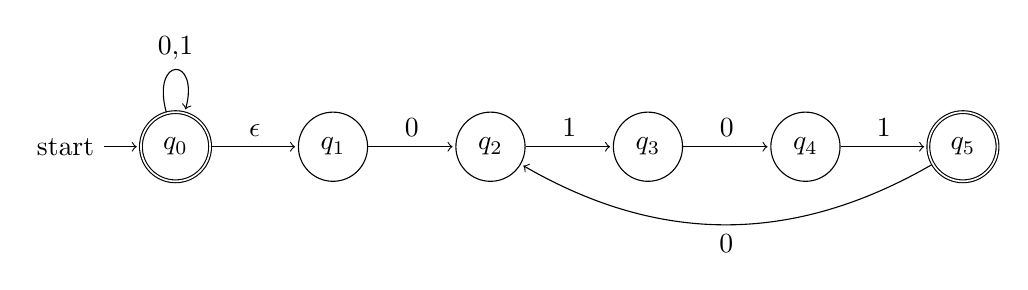
\begin{tikzpicture}[shorten >=1pt, node distance=2cm, on grid, auto]
    \node[state, initial, accepting] (q_0) {$q_0$};
    \node[state] (q_1) [right= of q_0] {$q_1$};
    \node[state] (q_2) [right= of q_1] {$q_2$};
    \node[state] (q_3) [right= of q_2] {$q_3$};
    \node[state] (q_4) [right= of q_3] {$q_4$};
    \node[state, accepting] (q_5) [right= of q_4] {$q_5$};
        \path[->]
        (q_0)   edge node {$\epsilon$} (q_1)
                edge [loop above] node {0,1} ()
        (q_1)   edge node {0} (q_2)
        (q_2)   edge node {1} (q_3)
        (q_3)   edge node {0} (q_4)
        (q_4)   edge node {1} (q_5)
        (q_5)   edge [bend left] node {0} (q_2);

\end{tikzpicture}

\newpage
Question 3)

\vspace{0.5cm}
M = ($\{q0,q1,q2,q3,q4,q5\}$,$\{0,1\}$,$\delta$,q0,$\{q0,q2,q4\}$)

where $\delta$ is 

\begin{center}
    \begin{tabular}{| l | l | l |}
    \hline
       & 0  & 1  \\ \hline
    q0 & q1 & q4 \\ \hline
    q1 & q2 & q3 \\ \hline
    q2 & q1 & q3 \\ \hline
    q3 & q3 & q3 \\ \hline
    q4 & q3 & q5 \\ \hline
    q5 & q3 & q4 \\
    \hline
    \end{tabular}
\end{center}

Question 4)

\vspace{0.5cm}
M = ($\{q0,q1,q2,q3,q4,q4,q5,q6,q7\}$,$\{0,1\}$,$\delta$,q0,$\{q7\}$)

where $\delta$ is 

\begin{center}
    \begin{tabular}{| l | l | l | l |}
    \hline
       & 0               & 1            & $\epsilon$   \\ \hline
    q0 & $\emptyset$     & q1           & $\emptyset$  \\ \hline
    q1 & q2              & $\emptyset$  & $\emptyset$  \\ \hline
    q2 & $\emptyset$     & q3           & $\emptyset$  \\ \hline
    q3 & q3              & q3           & q4           \\ \hline
    q4 & $\emptyset$     & q5           & $\emptyset$  \\ \hline
    q5 & q6              & $\emptyset$  & $\emptyset$  \\ \hline
    q6 & $\emptyset$     & q7           & $\emptyset$  \\ \hline
    q7 & $\emptyset$     & $\emptyset$  & $\emptyset$  \\
    \hline
    \end{tabular}
\end{center}

\newpage
Question 5
\newline
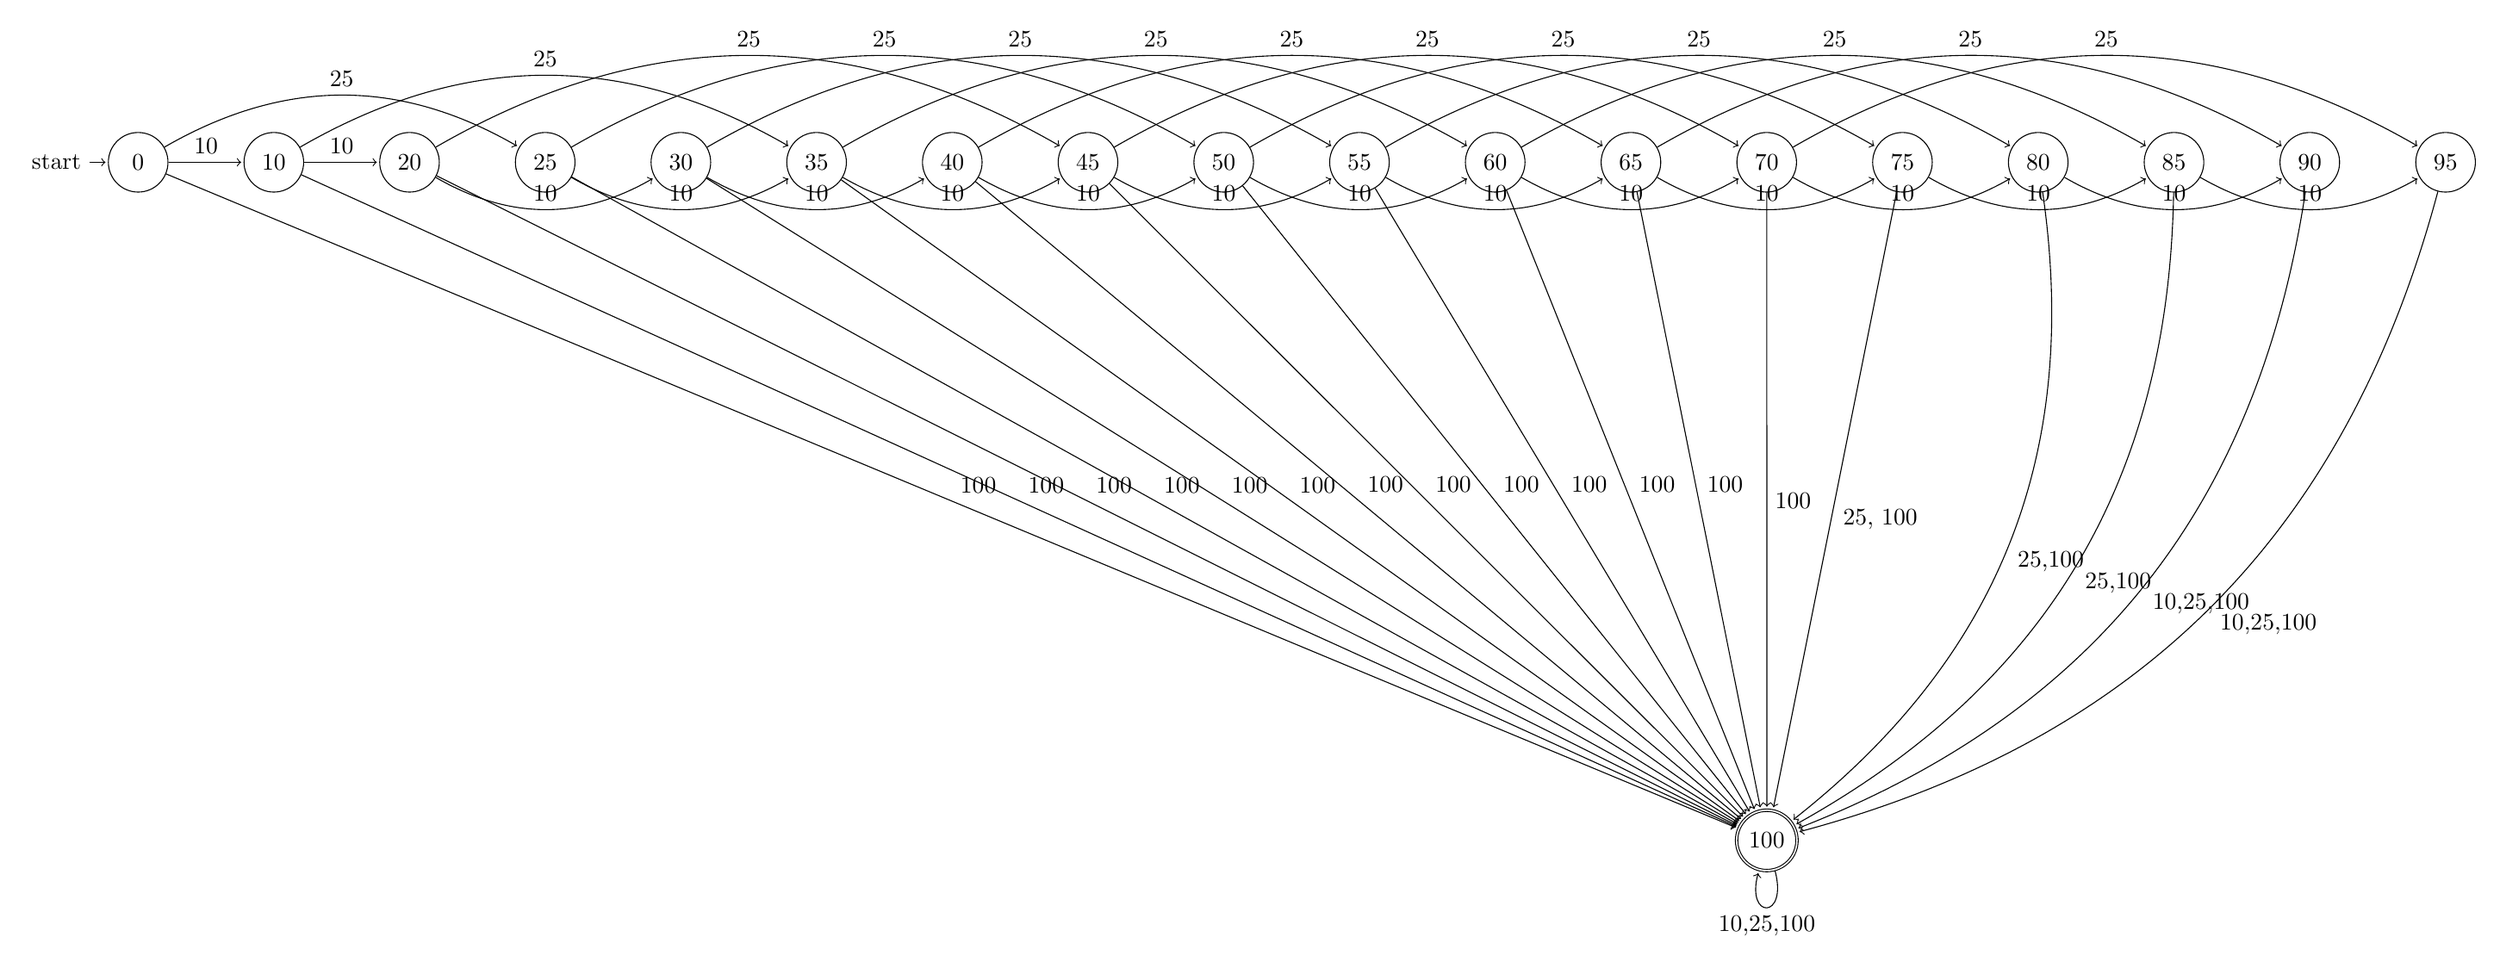
\begin{tikzpicture}[shorten >=1pt,scale=.6, node distance=2cm, on grid, auto ]
    \node[state, initial]   (0) {$0$};
    \node[state]            (10) [right= of 0] {$10$};
    \node[state]            (20) [right= of 10] {$20$};
    \node[state]            (25) [right= of 20] {$25$};
    \node[state]            (30) [right=  of 25] {$30$};
    \node[state]            (35) [right = of 30] {$35$};
    \node[state]            (40) [right  = of 35] {$40$};
    \node[state]            (45) [right  = of 40] {$45$};
    \node[state]            (50) [right =  of 45] {$50$};
    \node[state]            (55) [right=  of 50] {$55$};
    \node[state]            (60) [right= of 55] {$60$};
    \node[state]            (65) [right = of 60] {$65$};
    \node[state]            (70) [right = of 65] {$70$};
    \node[state]            (75) [right = of 70] {$75$};
    \node[state]            (80) [right =  of 75] {$80$};
    \node[state]            (85) [right = of 80] {$85$};
    \node[state]            (90) [right = of 85] {$90$};
    \node[state]            (95) [right  = of 90] {$95$};
    \node[state, accepting] (100)[ below  =10cm  of 70] {$100$};
        \path[->]
        (0)   edge node {10} (10)
              edge node {100}(100)
              edge [bend left] node {25}(25)
        (10)  edge node {10} (20)
              edge [bend left] node {25} (35)
              edge node {100}(100)
        (20)  edge [bend right] node {10} (30)
              edge [bend left] node {25} (45)
              edge node {100}(100)
        (25)  edge [bend right] node {10} (35)
              edge [bend left] node {25} (50)
              edge node {100}(100)
        (30)  edge [bend right] node {10} (40)
              edge [bend left] node {25} (55)
              edge node {100}(100)
        (35)  edge [bend right] node {10} (45)
              edge [bend left] node {25} (60)
              edge node {100}(100)
        (40)  edge [bend right] node {10} (50)
              edge [bend left] node {25} (65)
              edge node {100}(100)
        (45)  edge [bend right] node {10} (55)
              edge [bend left] node {25} (70)
              edge node {100}(100)
        (50)  edge [bend right] node {10} (60)
              edge [bend left] node {25} (75)
              edge node {100}(100)
        (55)  edge [bend right] node {10} (65)
              edge [bend left] node {25} (80)
              edge node {100}(100)
        (60)  edge [bend right] node {10} (70)
              edge [bend left] node {25} (85)
              edge node {100}(100)
        (65)  edge [bend right] node {10} (75)
              edge [bend left] node {25} (90)
              edge node {100}(100)
        (70)  edge [bend right] node {10} (80)
              edge [bend left] node {25} (95)
              edge node {100}(100)
        (75)  edge [bend right] node {10} (85)
              edge node {25, 100} (100)
        (80)  edge [bend right] node {10} (90)
              edge [bend left] node {25,100} (100)
        (85)  edge [bend right] node {10} (95)
              edge [bend left] node {25,100} (100)
        (90)  edge [bend left] node {10,25,100} (100)
        (95)  edge [bend left] node {10,25,100} (100)
        (100) edge [loop below] node {10,25,100} (100);
            
\newline
\newline
\newline
\newline
\end{tikzpicture}

\newpage
Question 5 (with 5c pieces)
\newline
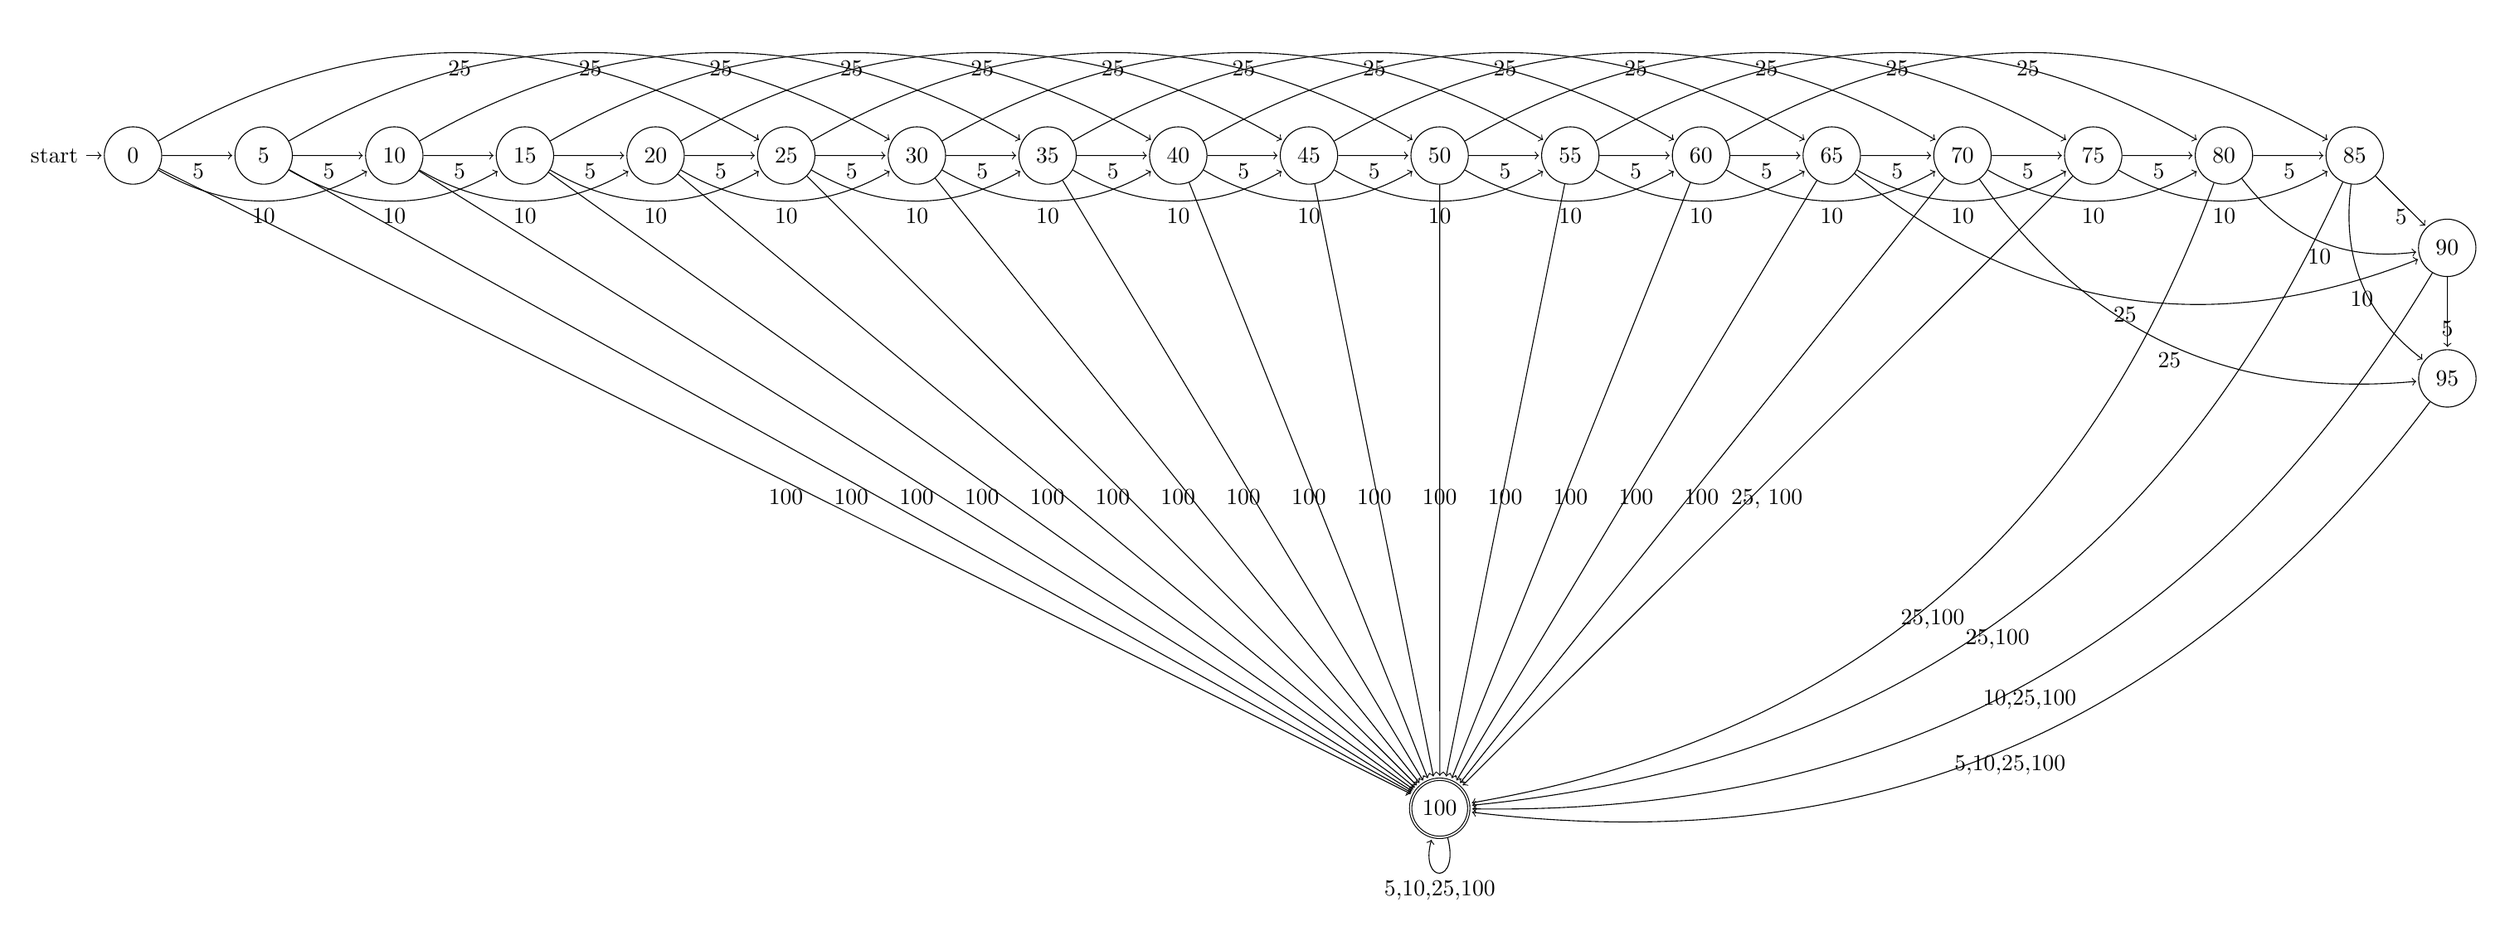
\begin{tikzpicture}[shorten >=1pt,scale=.6, node distance=2cm, on grid, below ]
\node[state, initial]   (0) {$0$};
\node[state]            (5) [right = of 0] {$5$};
\node[state]            (10) [right = of 5] {$10$};
\node[state]            (15) [right = of 10] {$15$};
\node[state]            (20) [right = of 15] {$20$};
\node[state]            (25) [right = of 20] {$25$};
\node[state]            (30) [right =  of 25] {$30$};
\node[state]            (35) [right = of 30] {$35$};
\node[state]            (40) [right = of 35] {$40$};
\node[state]            (45) [right = of 40] {$45$};
\node[state]            (50) [right = of 45] {$50$};
\node[state]            (55) [right = of 50] {$55$};
\node[state]            (60) [right = of 55] {$60$};
\node[state]            (65) [right = of 60] {$65$};
\node[state]            (70) [right = of 65] {$70$};
\node[state]            (75) [right = of 70] {$75$};
\node[state]            (80) [right = of 75] {$80$};
\node[state]            (85) [right = of 80] {$85$};
\node[state]            (90) [below right = of 85] {$90$};
\node[state]            (95) [below = of 90] {$95$};
\node[state, accepting] (100)[below  = 10cm  of 50] {$100$};
\path[->]
    (0)     edge node {5} (5)
            edge [bend right] node {10} (10)
            edge [bend left] node {25}(25)
            edge node {100}(100)
    (5)     edge node {5} (10)
            edge [bend right] node {10} (15)
            edge [bend left] node {25}(30)
            edge node {100}(100)
    (10)    edge node {5} (15)
            edge [bend right]node {10} (20)
            edge [bend left] node {25} (35)
            edge node {100}(100)
    (15)    edge node {5} (20)
            edge [bend right] node {10} (25)
            edge [bend left] node {25} (40)
            edge node {100}(100)        
    (20)    edge node {5} (25)
            edge [bend right] node {10} (30)
            edge [bend left] node {25} (45)
            edge node {100}(100)
    (25)    edge node {5} (30)
            edge [bend right] node {10} (35)
            edge [bend left] node {25} (50)
            edge node {100}(100)
    (30)    edge node {5} (35)
            edge [bend right] node {10} (40)
            edge [bend left] node {25} (55)
            edge node {100}(100)
    (35)    edge node {5} (40)
            edge [bend right] node {10} (45)
            edge [bend left] node {25} (60)
            edge node {100}(100)
    (40)    edge node {5} (45)
            edge [bend right] node {10} (50)
            edge [bend left] node {25} (65)
            edge node {100}(100)
    (45)    edge node {5} (50)
            edge [bend right] node {10} (55)
            edge [bend left] node {25} (70)
            edge node {100}(100)
    (50)    edge node {5} (55)
            edge [bend right] node {10} (60)
            edge [bend left] node {25} (75)
            edge node {100}(100)
    (55)    edge node {5} (60)
            edge [bend right] node {10} (65)
            edge [bend left] node {25} (80)
            edge node {100}(100)
    (60)    edge node {5} (65)
            edge [bend right] node {10} (70)
            edge [bend left] node {25} (85)
            edge node {100}(100)
    (65)    edge node {5} (70)
            edge [bend right] node {10} (75)
            edge [bend right] node {25} (90)
            edge node {100}(100)
    (70)    edge node {5} (75)
            edge [bend right] node {10} (80)
            edge [bend right] node {25} (95)
            edge node {100}(100)
    (75)    edge node {5} (80)
            edge [bend right] node {10} (85)
            edge node {25, 100} (100)
    (80)    edge node {5} (85)
            edge [bend right] node {10} (90)
            edge [bend left] node {25,100} (100)
    (85)    edge node {5} (90)
            edge [bend right] node {10} (95)
            edge [bend left] node {25,100} (100)
    (90)    edge node {5} (95)
            edge [bend left] node {10,25,100} (100)
    (95)    edge [bend left] node {5,10,25,100} (100)
    (100)   edge [loop below] node {5,10,25,100} (100);

\newline
\newline
\newline
\newline
\end{tikzpicture}

\newpage
Question 6)
\newline
\newline
\newline
\vspace{2cm}
\begin{tikzpicture}[shorten >=1pt, node distance=8cm, on grid, auto]
    \node[state, initial, accepting] (q_0) {$q_0$};
    \node[state] (q_1) [below right of = q_0] {$q_1$};
    \node[state, accepting] (q_2) [above right of = q_0] {$q_2$};
        \path[->]
        (q_0)   edge node {$
                            \begin{bmatrix}
                            0 \\
                            1
                            \end{bmatrix}
                             $} (q_1)
                edge [loop above] node {$
                                        \begin{bmatrix}
                                        0 \\ 
                                        0 
                                        \end{bmatrix},
                                        \begin{bmatrix}
                                        1 \\ 
                                        1 
                                        \end{bmatrix}
                                        $} ()
                edge node {$
                      \begin{bmatrix}
                      1 \\
                      0
                      \end{bmatrix}
                      $} (q_2)
        (q_1)   edge [loop below] node {$
                                        \begin{bmatrix}
                                        1 \\ 
                                        1 
                                        \end{bmatrix},
                                        \begin{bmatrix}
                                        1 \\ 
                                        0 
                                        \end{bmatrix},
                                        \begin{bmatrix}
                                        0 \\ 
                                        1 
                                        \end{bmatrix},
                                        \begin{bmatrix}
                                        0 \\ 
                                        0 
                                        \end{bmatrix}
                                        $} ()
        (q_2)   edge [loop above] node {$
                                        \begin{bmatrix}
                                        1 \\ 
                                        1 
                                        \end{bmatrix},
                                        \begin{bmatrix}
                                        1 \\ 
                                        0 
                                        \end{bmatrix},
                                        \begin{bmatrix}
                                        0 \\ 
                                        1 
                                        \end{bmatrix},
                                        \begin{bmatrix}
                                        0 \\ 
                                        0 
                                        \end{bmatrix}
                                        $} ();

\end{tikzpicture}

\newpage
Question 7)
$L_1 - L_2 = L_1 \cap \overline{L_2}$

Since $L_1$ is regular, $\overline{L_2}$ (complement of $L_2$) is regular and intersection are all closed under the set of regular languages then $L_1 \cap \overline{L_2}$ is regular.


\vspace{8cm}
Question 8)
We assume that ADD is regular.

Let p be the puming length given by the pumping lemma

we let s be the string

$1^p = 0 + 1^p$

Because $s \in B \land s > p$ we guarentee that $s$ can be split into three piece $s = xyz$
\newline
where these three things must hold 
\newline
i) $xy^iz \in ADD    ,i>=0
\newline
ii) |xy| <= p
\newline
iii) |y| > 0$


Suppose y contains only 1's

let $y = 1^m$ such that $m >= 1$

$
xy = 1^p\newline
x = 1^{p-m}\newline
z = ( = 0 + 1^p)
$
\newline
$
xyz     (1^{p-m})(1^m)(= 0 + 1^p)
$
\newline
suppose $i = 0$
\newline
$
xy^iz = (1^{p-m}(1^m)^0( = 0 + 1^p)
\newline
      = 1^{p-m} = 0 + 1^p
$
\newline
if $m>=1, p-m \neq p$

Hence $\exists i$ such that $xy^iz \notin ADD$


\newpage
Question 9)

a)\newline
Accept:\newline
a\newline
b

Reject:\newline
ba\newline
bbaa


b)\newline
Accept:\newline
a\newline 
aba\newline  

Reject:\newline
b\newline 
ba\newline 


c)\newline
Accept:\newline
a\newline 
bb  

Reject:\newline
aa\newline  
aab\newline  


d)\newline
Accept:\newline
$\epsilon$b\newline 
ab 

Reject:\newline
aab\newline
bb
\end{document}
